% !TeX root = ../sdc_regulations.tex
% Add the above to each chapter to make compiling the PDF easier for some editors.

\newpage

\begin{note}
\textbf{NOTE:} This is a rough outline for a capture the flag style competition. It is highly adaptable in terms of
\begin{itemize}
    \item {amount and layoout of the areas}
    \item {adding obstacles to the field}
    \item {adding rules like "only adjacent areas can be activated" or "camping is prohibited"}
\end{itemize}

\vspace{5mm}
For safety, I introduced a separation rule similar to the semi-circular rule in general aviation.

\vspace{5mm}
The game forces the participants to
\begin{itemize}
    \item {Coordinate the actions of the drones, since it takes at least two drones to activate an area}
    \item {Identify the areas}
    \item {Check if the area is occupied by other drones}
    \item {Identify and land designated landing pads on the areas}
    \item {Keep separation when moving over the field by staying within a certain height}
\end{itemize}

\vspace{5mm}
The game might require either a jury watching the field, which might be a bit difficult with up to 16 drones at once. Better would be a visual based tracking of the vehicles with a shared info space where a) the activation of the areas can be tracked and b) the participants can see the state of the areas (neutral, activated by own, activated by other).

\vspace{5mm}
The outline does not touch technical topics as in "level of autonomy", "human interaction" or such.
\end{note}
    
\newpage

\section{The Game}

\begin{quote}
    The supreme art of war is to subdue the enemy without fighting. 
    \begin{flushright}
        -- Sun Tzu, \textit{The Art of War}
    \end{flushright}
\end{quote}

\subsection{Description}
This is a capture the flag style game with multiple areas that are spread accross the playfield. The areas start as neutral and can be occupied / activated or won back. Activating or neutralizing an area will get you points, as well as holding an area for a certain period of time. You can also prevent areas from being neutralized again, by keeping it occupied with at least one drone.

\subsection{The Playfield}
The playfield is 48m x 18m and can be used up to a height of 6m.
\begin{figure}[h]
    \centering
    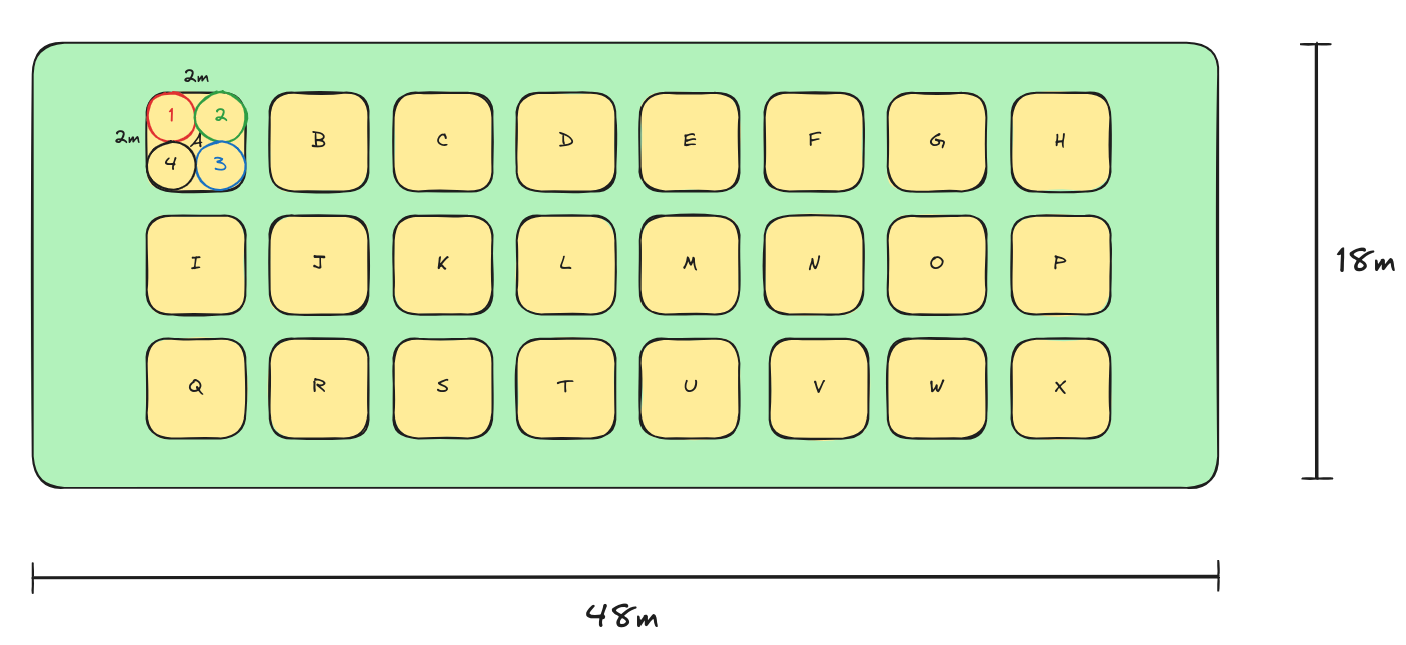
\includegraphics[width=0.8\textwidth]{figures/field.png}
    \caption{The playfield}
    \label{fig:playfield}
\end{figure}

\subsection{Areas}
Accross the playfield there is the areas that can be occupied. Each area is 2m x 2m, labled with a letter and has 4 designated landing pads. The landing pads are labled from 1..4, starting at the top left corner and then going clockwise.
\begin{figure}[h]
    \centering
    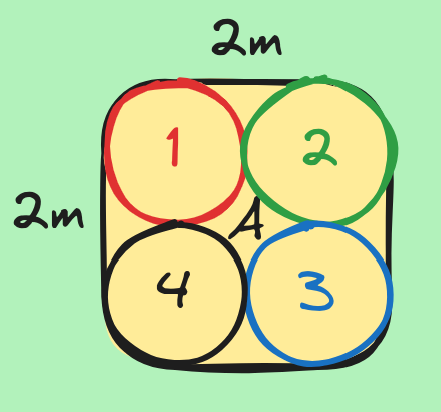
\includegraphics[width=0.3\textwidth]{figures/area.png}
    \caption{An area}
    \label{fig:area}
\end{figure}

\newpage
\subsection{Game Dynamics}
Aim of the game is to activate and keep as many areas for as long as possible.
\begin{enumerate}
	\item {All areas start as neutral.}
	\item {To activate an area, it must be occupied by at least 2 drones for 5 seconds.}
	\item {Areas that are activated by the opposing team need to be neutralized first.}
    \item {To neutralize an area, it must be occupied by at least 2 drones for 5 seconds.}
    \item {Only areas that are free of opposing drones can be neutralized}
\end{enumerate}

\subsection{Separation}
For better separation / collision avoidance, the UAVs shall move within a certain height. When moving from left to right, they shall stay within 0m .. 2m and when moving from right to left, they shall stay within 4m..6m. This leaves plenty of space to avoid head on collision.
\begin{figure}[h]
\centering
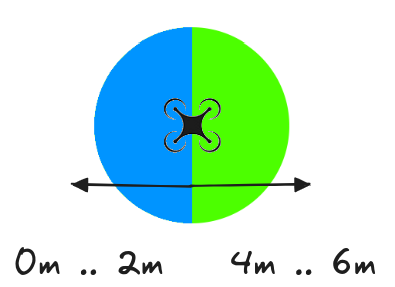
\includegraphics[width=0.2\textwidth]{figures/separation.png}
\caption{Semicircular separation}
\label{fig:separation}
\end{figure}

\subsection{Scoring}
\begin{center}
    \begin{tabular}{|c|l|c|}
        \hline
        ID & Description & Score \\
        \hline
        1 & Activating an area & 10 \\
        \hline
        2 & Neutralizing an area & 10 \\
        \hline
        3 & Holding an area for 10s & 10 \\
        \hline
        4 & Violating the Separation Rule & -50 \\
        \hline
    \end{tabular}
\end{center}
